\chapter{Appendix}

\begin{figure}[H]
\centering
\caption{Each line represents one convolution layer in the VGG13\_bn architecture is ascending order. Four interesting activations are shown per layer.}
\subfigure{

\includegraphics[width=.23\textwidth]{images/chapter5/vgg13-bn/l0-f0.jpg}
}
\subfigure{

\includegraphics[width=.23\textwidth]{images/chapter5/vgg13-bn/l0-f1.jpg}
}
\subfigure{

\includegraphics[width=.23\textwidth]{images/chapter5/vgg13-bn/l0-f2.jpg}
}
\subfigure{

\includegraphics[width=.23\textwidth]{images/chapter5/vgg13-bn/l0-f3.jpg}
}

\subfigure{
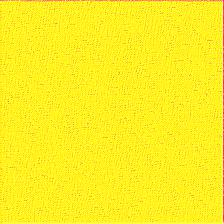
\includegraphics[width=.23\textwidth]{images/chapter5/vgg13-bn/l3-f0.jpg}
}
\subfigure{
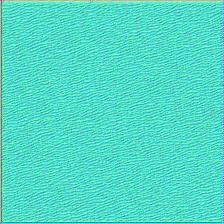
\includegraphics[width=.23\textwidth]{images/chapter5/vgg13-bn/l3-f1.jpg}
}
\subfigure{

\includegraphics[width=.23\textwidth]{images/chapter5/vgg13-bn/l3-f2.jpg}
}
\subfigure{
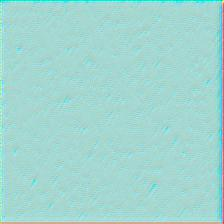
\includegraphics[width=.23\textwidth]{images/chapter5/vgg13-bn/l3-f3.jpg}
}

\subfigure{
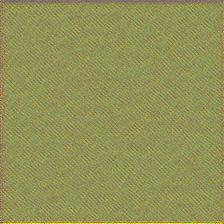
\includegraphics[width=.23\textwidth]{images/chapter5/vgg13-bn/l7-f0.jpg}
}
\subfigure{

\includegraphics[width=.23\textwidth]{images/chapter5/vgg13-bn/l7-f1.jpg}
}
\subfigure{

\includegraphics[width=.23\textwidth]{images/chapter5/vgg13-bn/l7-f2.jpg}
}
\subfigure{
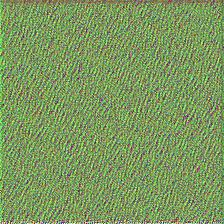
\includegraphics[width=.23\textwidth]{images/chapter5/vgg13-bn/l7-f3.jpg}
}

\subfigure{
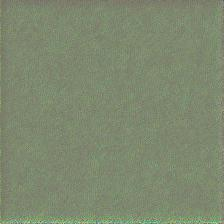
\includegraphics[width=.23\textwidth]{images/chapter5/vgg13-bn/l10-f0.jpg}
}
\subfigure{

\includegraphics[width=.23\textwidth]{images/chapter5/vgg13-bn/l10-f1.jpg}
}
\subfigure{
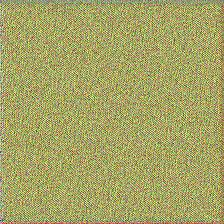
\includegraphics[width=.23\textwidth]{images/chapter5/vgg13-bn/l10-f2.jpg}
}
\subfigure{

\includegraphics[width=.23\textwidth]{images/chapter5/vgg13-bn/l10-f3.jpg}
}

\subfigure{

\includegraphics[width=.23\textwidth]{images/chapter5/vgg13-bn/l14-f0.jpg}
}
\subfigure{

\includegraphics[width=.23\textwidth]{images/chapter5/vgg13-bn/l14-f1.jpg}
}
\subfigure{

\includegraphics[width=.23\textwidth]{images/chapter5/vgg13-bn/l14-f2.jpg}
}
\subfigure{

\includegraphics[width=.23\textwidth]{images/chapter5/vgg13-bn/l14-f3.jpg}
}

\subfigure{

\includegraphics[width=.23\textwidth]{images/chapter5/vgg13-bn/l17-f0.jpg}
}
\subfigure{

\includegraphics[width=.23\textwidth]{images/chapter5/vgg13-bn/l17-f1.jpg}
}
\subfigure{

\includegraphics[width=.23\textwidth]{images/chapter5/vgg13-bn/l17-f2.jpg}
}
\subfigure{

\includegraphics[width=.23\textwidth]{images/chapter5/vgg13-bn/l17-f3.jpg}
}

\subfigure{

\includegraphics[width=.23\textwidth]{images/chapter5/vgg13-bn/l21-f0.jpg}
}
\subfigure{

\includegraphics[width=.23\textwidth]{images/chapter5/vgg13-bn/l21-f1.jpg}
}
\subfigure{

\includegraphics[width=.23\textwidth]{images/chapter5/vgg13-bn/l21-f2.jpg}
}
\subfigure{

\includegraphics[width=.23\textwidth]{images/chapter5/vgg13-bn/l21-f3.jpg}
}

\subfigure{

\includegraphics[width=.23\textwidth]{images/chapter5/vgg13-bn/l24-f0.jpg}
}
\subfigure{

\includegraphics[width=.23\textwidth]{images/chapter5/vgg13-bn/l24-f1.jpg}
}
\subfigure{

\includegraphics[width=.23\textwidth]{images/chapter5/vgg13-bn/l24-f2.jpg}
}
\subfigure{

\includegraphics[width=.23\textwidth]{images/chapter5/vgg13-bn/l24-f3.jpg}
}

\subfigure{

\includegraphics[width=.23\textwidth]{images/chapter5/vgg13-bn/l28-f0.jpg}
}
\subfigure{

\includegraphics[width=.23\textwidth]{images/chapter5/vgg13-bn/l28-f1.jpg}
}
\subfigure{

\includegraphics[width=.23\textwidth]{images/chapter5/vgg13-bn/l28-f2.jpg}
}
\subfigure{

\includegraphics[width=.23\textwidth]{images/chapter5/vgg13-bn/l28-f3.jpg}
}

\subfigure{

\includegraphics[width=.23\textwidth]{images/chapter5/vgg13-bn/l31-f0.jpg}
}
\subfigure{

\includegraphics[width=.23\textwidth]{images/chapter5/vgg13-bn/l31-f1.jpg}
}
\subfigure{

\includegraphics[width=.23\textwidth]{images/chapter5/vgg13-bn/l31-f2.jpg}
}
\subfigure{

\includegraphics[width=.23\textwidth]{images/chapter5/vgg13-bn/l31-f3.jpg}
}

\label{fig:vgg13_app_fromscratch_filters}
\end{figure}

\begin{figure}[H]
\centering
\caption{Each line represents one convolution layer in the VGG13\_bn architecture is ascending order. Four interesting activations are shown per layer.}
\subfigure{

\includegraphics[width=.23\textwidth]{images/chapter5/vgg13-bn-pre/l0-f0.jpg}
}
\subfigure{

\includegraphics[width=.23\textwidth]{images/chapter5/vgg13-bn-pre/l0-f1.jpg}
}
\subfigure{

\includegraphics[width=.23\textwidth]{images/chapter5/vgg13-bn-pre/l0-f2.jpg}
}
\subfigure{

\includegraphics[width=.23\textwidth]{images/chapter5/vgg13-bn-pre/l0-f3.jpg}
}

\subfigure{
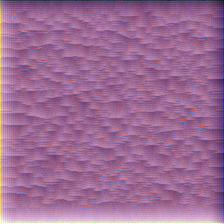
\includegraphics[width=.23\textwidth]{images/chapter5/vgg13-bn-pre/l3-f0.jpg}
}
\subfigure{
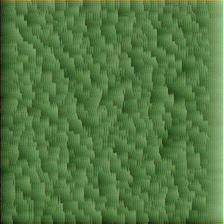
\includegraphics[width=.23\textwidth]{images/chapter5/vgg13-bn-pre/l3-f1.jpg}
}
\subfigure{

\includegraphics[width=.23\textwidth]{images/chapter5/vgg13-bn-pre/l3-f2.jpg}
}
\subfigure{
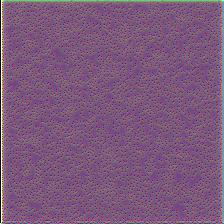
\includegraphics[width=.23\textwidth]{images/chapter5/vgg13-bn-pre/l3-f3.jpg}
}

\subfigure{
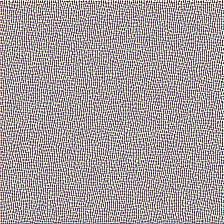
\includegraphics[width=.23\textwidth]{images/chapter5/vgg13-bn-pre/l7-f0.jpg}
}
\subfigure{

\includegraphics[width=.23\textwidth]{images/chapter5/vgg13-bn-pre/l7-f1.jpg}
}
\subfigure{
\includegraphics[width=.23\textwidth]{images/chapter5/vgg13-bn-pre/l7-f2.jpg}
}
\subfigure{
\includegraphics[width=.23\textwidth]{images/chapter5/vgg13-bn-pre/l7-f3.jpg}
}

\subfigure{
\includegraphics[width=.23\textwidth]{images/chapter5/vgg13-bn-pre/l10-f0.jpg}
}
\subfigure{
\includegraphics[width=.23\textwidth]{images/chapter5/vgg13-bn-pre/l10-f1.jpg}
}
\subfigure{
\includegraphics[width=.23\textwidth]{images/chapter5/vgg13-bn-pre/l10-f2.jpg}
}
\subfigure{
\includegraphics[width=.23\textwidth]{images/chapter5/vgg13-bn-pre/l10-f3.jpg}
}

\subfigure{
\includegraphics[width=.23\textwidth]{images/chapter5/vgg13-bn-pre/l14-f0.jpg}
}
\subfigure{
\includegraphics[width=.23\textwidth]{images/chapter5/vgg13-bn-pre/l14-f1.jpg}
}
\subfigure{
\includegraphics[width=.23\textwidth]{images/chapter5/vgg13-bn-pre/l14-f2.jpg}
}
\subfigure{
\includegraphics[width=.23\textwidth]{images/chapter5/vgg13-bn-pre/l14-f3.jpg}
}

\subfigure{
\includegraphics[width=.23\textwidth]{images/chapter5/vgg13-bn-pre/l17-f0.jpg}
}
\subfigure{
\includegraphics[width=.23\textwidth]{images/chapter5/vgg13-bn-pre/l17-f1.jpg}
}
\subfigure{
\includegraphics[width=.23\textwidth]{images/chapter5/vgg13-bn-pre/l17-f2.jpg}
}
\subfigure{
\includegraphics[width=.23\textwidth]{images/chapter5/vgg13-bn-pre/l17-f3.jpg}
}

\subfigure{
\includegraphics[width=.23\textwidth]{images/chapter5/vgg13-bn-pre/l21-f0.jpg}
}
\subfigure{
\includegraphics[width=.23\textwidth]{images/chapter5/vgg13-bn-pre/l21-f1.jpg}
}
\subfigure{
\includegraphics[width=.23\textwidth]{images/chapter5/vgg13-bn-pre/l21-f2.jpg}
}
\subfigure{
\includegraphics[width=.23\textwidth]{images/chapter5/vgg13-bn-pre/l21-f3.jpg}
}

\subfigure{
\includegraphics[width=.23\textwidth]{images/chapter5/vgg13-bn-pre/l24-f0.jpg}
}
\subfigure{
\includegraphics[width=.23\textwidth]{images/chapter5/vgg13-bn-pre/l24-f1.jpg}
}
\subfigure{
\includegraphics[width=.23\textwidth]{images/chapter5/vgg13-bn-pre/l24-f2.jpg}
}
\subfigure{
\includegraphics[width=.23\textwidth]{images/chapter5/vgg13-bn-pre/l24-f3.jpg}
}

\subfigure{
\includegraphics[width=.23\textwidth]{images/chapter5/vgg13-bn-pre/l28-f0.jpg}
}
\subfigure{
\includegraphics[width=.23\textwidth]{images/chapter5/vgg13-bn-pre/l28-f1.jpg}
}
\subfigure{
\includegraphics[width=.23\textwidth]{images/chapter5/vgg13-bn-pre/l28-f2.jpg}
}
\subfigure{
\includegraphics[width=.23\textwidth]{images/chapter5/vgg13-bn-pre/l28-f3.jpg}
}

\subfigure{
\includegraphics[width=.23\textwidth]{images/chapter5/vgg13-bn-pre/l31-f0.jpg}
}
\subfigure{
\includegraphics[width=.23\textwidth]{images/chapter5/vgg13-bn-pre/l31-f1.jpg}
}
\subfigure{
\includegraphics[width=.23\textwidth]{images/chapter5/vgg13-bn-pre/l31-f2.jpg}
}
\subfigure{
\includegraphics[width=.23\textwidth]{images/chapter5/vgg13-bn-pre/l31-f3.jpg}
}

\label{fig:vgg13_app_pretrained_filters}
\end{figure}